\chapter{Results}
In this chapter we will present the results coming from the process of parameter adjustment and the results coming from the final evaluation. During the parameter adjustment we use as an input for our neural network, EMG data with the Myo armband coming from the forearm regarding extension and flexion of the thumb. For the evaluation stage we acquired EMG signals from 21 subjects regarding extension and flexions of different gestures. 
\section{Parameter adjustment}
The first experiment we ran had the purpose to find the best average accuracies for the detection between thumb extension and flexion per feature.
\begin{figure}[h!]
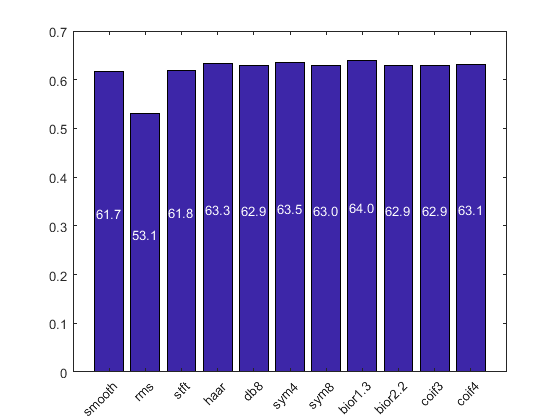
\includegraphics[width=15cm,left,keepaspectratio]{figures/HL1HN5step1}
\caption{Average performances with one hidden layer, five neurons and step one}
\label{fig:HL1HN5step1}
\end{figure}
As fig. \ref{fig:HL1HN5step1} shows, we have estimated the average accuracies for the training and testing of each of the 55 folds of data we have created. The best accuracy was from the discrete wavelet bior1.3 which gave $64 \%$ detection accuracy and the worst performance was from the root-mean-square with $53.1 \%$.\\
The time for training the model and testing it for the existing amount of data has found to be prohibitively long. Therefore, due to the large quantity of data we chose for the next experiments to decrease the amount of it by increasing the step of the windowing from 1 to 64. The second experiment had the purpose to check whether the neural net with one hidden layer and five hidden nodes can give us similar or better results with less data.
\begin{figure}[h!]
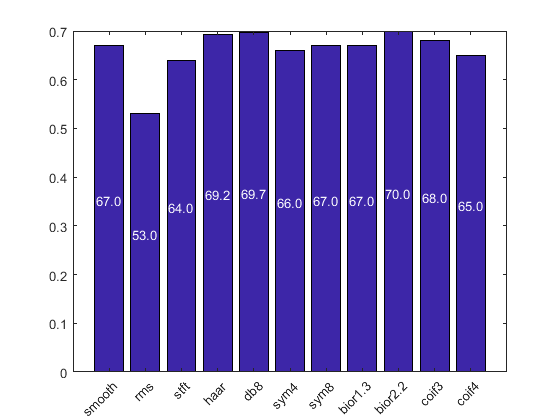
\includegraphics[width=15cm,left,keepaspectratio]{figures/HL1HN5step64}
\caption{Average performances with one hidden layer, five neurons and step 64}
\label{fig:HL1HN5step64}
\end{figure}
Fig. \ref{fig:HL1HN5step64} shows slightly better results than the first batch. As we can observe in almost every feature we got better results with less data.\\
For the next experiment we decided to combine all possible combinations of the train and test data extracted  with the window step of 64 produced from the different features we selected for the current work. In total, we have 11  features and each feature has five folds for the training data and five folds for the test data. Combining all 11 features in groups of two then there are 55 combinations which is calculated by the following equation:
\begin{equation}
\binom{n}{k} = \frac{n(n-1) \cdots (n-k+1)}{k(k-1) \cdots 1} = \frac{n!}{k!(n-k)!}
\end{equation}
Taking into account that each combination is accompanied by five folds of training and test data it means that we will run $55 \times 5 = 275$ neural nets. The overall runtime of the whole experiment was $5.8$ days. The average time for one experiment was $30.7$ minutes.
In Table \ref{table:perf_features_duet} we can see the results of the average detection accuracies between extension and flexion of the thumb from testing the trained neural nets with one hidden layer and five hidden neurons. The best performances are highlighted with blue color.
\begin{table}
\renewcommand{\arraystretch}{1.2}
\begin{tabular}{ |p{1.3cm}||p{1cm}|p{1cm}|p{1cm}|p{1cm}|p{1cm}|p{1cm}|p{1.1cm}|p{1.1cm}|p{1cm}|p{1cm}|  }
 \hline
 \multicolumn{11}{|c|}{Average accuracies from the combinations of all features} \\
 \hline
 Features  & rms & stft & haar & db8 & sym4 & sym8 & bior1.3 & bior2.2 & coif3 & coif4\\
 \hline
 smooth   & $64.4\%$ &$63.0\%$ &$58.9\%$ &$65.4\%$ &$63.7\%$ &$67.1\%$ &$67.4\%$ &$65.3\%$ &$66.2\%$ &$69.3\%$ \\
 rms & - &$66.1\%$ &$61.7\%$ &$69.2\%$ &$62.9\%$ &\cellcolor{blue!35}$69.9\%$ &\cellcolor{blue!35}$70.0\%$ &$63.1\%$ &$69.0\%$ &$68.0\%$\\
 stft & - & - & $67.0\%$ &$61.6\%$ &$66.3\%$ &$60.9\%$ &$68.8\%$ &$67.9\%$ &$62.4\%$ &$63.0\%$\\
 haar & - & - & - & $67.9\%$ &$66.9\%$ &$64.0\%$ &$66.3\%$ &$62.7\%$ &$63.1\%$ &$64.8\%$\\
 db8 & - & - & - & - &$69.2\%$ &$66.7\%$ &$68.7\%$ &$59.5\%$ &$66.4\%$ &$65.8\%$\\
 sym4 & - & - & - & - & - &\cellcolor{blue!35}$70.3\%$ &$68.2\%$ &$62.0\%$ &$67.8\%$ &$66.1\%$\\
 sym8 & - & - & - & - & - & - &$66.8\%$ &$59.4\%$ &$64.2\%$ &$64.7\%$\\
 bior1.3 & - & - & - & - & - & - & - &$66.8\%$ &$69.4\%$ &$59.5\%$\\
 bior2.2 & - & - & - & - & - & - & - & - &$69.3\%$ &$65.7\%$\\
 coif3 & - & - & - & - & - & - & - & - & - &$65.9\%$\\
 \hline
\end{tabular}
\caption{Combined features and ran on neural net with one hidden layer and five hidden neurons.}
\label{table:perf_features_duet}
\end{table}
From the Table \ref{table:perf_features_duet} we can see that the best performance is when we combine the features sym4 with sym8. For the next step we decided to concatenate the sym4 with sym8 and combine their concatenation with each and every other feature from the feature set.  \\
In Table \ref{table:sym4sym8} we can see the average performances per 3 features for classification in one hidden layer and five hidden neurons network.
\begin{table}[h!]
\renewcommand{\arraystretch}{1.3}
\begin{tabular}{ |p{1.6cm}||p{1.2cm}|p{1cm}|p{1cm}|p{1cm}|p{1cm}|p{1.1cm}|p{1.1cm}|p{1cm}|p{1cm}|  }
 \hline
 \multicolumn{10}{|c|}{Average accuracies from the combinations of all features} \\
 \hline
 Features  & smooth & rms & stft & haar & db8 & bior1.3 & bior2.2 & coif3 & coif4\\
 \hline
 sym4sym8  & $58.0\%$ &$61.0\%$ &$65.1\%$ &$65.2\%$ &$64.5\%$ &$65.7\%$ &\cellcolor{blue!35}$68.7\%$ &\cellcolor{blue!35}$68.4\%$ &$67.9\%$\\
 \hline
\end{tabular}
\caption{Combined features per 3 and ran on neural net with one hidden layer and five hidden neurons.}
\label{table:sym4sym8}
\end{table}
For the next experiment we chose the second best performance from the Table \ref{table:perf_features_duet} which was between the rms and sym8. We concatenated the two features and again tested against every other feature. The Table \ref{table:rmssym8} show us the results:
\begin{table}[h!]
\renewcommand{\arraystretch}{1.3}
\begin{tabular}{ |p{1.6cm}||p{1.2cm}|p{1cm}|p{1cm}|p{1cm}|p{1cm}|p{1.1cm}|p{1.1cm}|p{1cm}|p{1cm}|  }
 \hline
 \multicolumn{10}{|c|}{Average accuracies from the combinations of all features} \\
 \hline
 Features  & smooth & stft & haar & db8 &sym4 & bior1.3 & bior2.2 & coif3 & coif4\\
 \hline
 rmssym8  & $58.1\%$ &\cellcolor{blue!35}$64.8\%$ &$59.7\%$ &$57.9\%$ &$62.1\%$ &$58.2\%$ &$62.0\%$ &$60.3\%$ &\cellcolor{blue!35}$63.3\%$\\
 \hline
\end{tabular}
\caption{Combined features per 3 and ran on neural net with one hidden layer and five hidden neurons.}
\label{table:rmssym8}
\end{table}
\newpage
For the next experiment we chose the third best performance from the Table \ref{table:perf_features_duet} which was between between the rms and bior1.3. Again, we concatenated these two features and tested against every other feature. The Table \ref{table:rmsbior13} show us the results:
\begin{table}[h!]
\renewcommand{\arraystretch}{1.3}
\begin{tabular}{ |p{1.6cm}||p{1.2cm}|p{1cm}|p{1cm}|p{1cm}|p{1cm}|p{1cm}|p{1.1cm}|p{1cm}|p{1cm}|  }
 \hline
 \multicolumn{10}{|c|}{Average accuracies from the combinations of all features} \\
 \hline
 Features  & smooth & stft & haar & db8 & sym4 & sym8 & bior2.2 & coif3 & coif4\\
 \hline
 rmsbior1.3  & $61.9\%$ &$62.3\%$ &\cellcolor{blue!35}$65.8\%$ &$62.9\%$ &$61.8\%$ &$63.3\%$ &$62.9\%$ &$62.8\%$ &\cellcolor{blue!35}$64.8\%$\\
 \hline
\end{tabular}
\caption{Combined features per 3 and ran on neural net with one hidden layer and five hidden neurons.}
\label{table:rmsbior13}
\end{table}
For the next experiment, we decided to concatenate the duplet of sym4 and sym8 and test it against all the other features and also incrementing the number of layers from one to eight layers with each consisting of 5 hidden neurons. The total number of nets that had to be trained was 585. The duration of this experiment was 73 days. The average time for each training and classification was 2.9 hours. The Table \ref{table:sym4sym8_1-5layers} shows us the results:
\begin{table}[h!]
\renewcommand{\arraystretch}{1.2}
\begin{tabular}{ |p{1.7cm}||p{1.2cm}|p{1cm}|p{1cm}|p{1cm}|p{1cm}|p{1.1cm}|p{1.1cm}|p{1cm}|p{1cm}|}
 \hline
 \multicolumn{10}{|c|}{sym4sym8} \\
 \hline
 Layers  & smooth & rms & stft & haar & db8 & bior1.3 & bior2.2 & coif3 & coif4\\
 \hline
 1 Layer  & \cellcolor{blue!35}$68.1\%$ & $61.0\%$ &$63.5\%$ &\cellcolor{blue!35}$67.0\%$ &$61.0\%$ &\cellcolor{blue!35}$68.0\%$ &$66.0\%$ &$64.4\%$ &$66.0\%$\\
 2 Layers & \cellcolor{blue!35}$69.7\%$ & $66.0\%$ &\cellcolor{blue!35}$70.5\%$ &$68.4\%$ &$69.2\%$ &$67.1\%$ &\cellcolor{blue!35}$69.5\%$ &$68.4\%$ & $67.0\%$\\
 3 Layers &\cellcolor{blue!35} $67.0\%$ & $63.7\%$ & $72.4\%$ & $70.0\%$ &$68.4\%$ &\cellcolor{blue!35}$71.2\%$ &$69.7\%$ &$69.1\%$ &\cellcolor{blue!35}$70.7\%$\\
 4 Layers & \cellcolor{blue!35}$72.0\%$ & $65.0\%$ & $71.4\%$ & $71.5\%$ &\cellcolor{blue!35}$72.1\%$ &$71.1\%$ &$70.5\%$ &$69.4\%$ &\cellcolor{blue!35}$73.0\%$\\
 5 Layers & $71.3\%$ & $67.8\%$ &\cellcolor{blue!35}$74.0\%$ &\cellcolor{blue!35}$72.5\%$ &$71.0\%$ &$71.5\%$ &\cellcolor{blue!35}$72.5\%$ &$70.5\%$ &$67.0\%$\\
 6 Layers & \cellcolor{blue!35}$74.2\%$ & $71.1\%$ & $73.0\%$ & \cellcolor{blue!35}$73.8\%$ &\cellcolor{blue!35}$74.2\%$ &$72.6\%$ &$74.1\%$ &$72.3\%$ &$71.5\%$\\
 7 Layers & $73.2\%$ & $68.6\%$ & \cellcolor{blue!35}$74.0\%$ & $73.5\%$ &$71.7\%$ &$73.0\%$ &\cellcolor{blue!35}$74.3\%$ &\cellcolor{blue!35}$73.8\%$ &$73.2\%$\\
 8 Layers &$72.9\%$ & $71.0\%$ & $72.3\%$ & $72.2\%$ &\cellcolor{blue!35}$73.5\%$ &\cellcolor{blue!35}$73.6\%$ &$73.5\%$ & \cellcolor{blue!35}$74.3\%$ &$72.0\%$\\
 9 Layers & \cellcolor{blue!35}$74.2\%$ & $63.2\%$ & \cellcolor{blue!35}$74.8\%$ & $72.8\%$ &$74.0\%$ &$73.5\%$ &$72.1\%$ & \cellcolor{blue!35}$74.4\%$ &$71.5\%$\\
 10 Layers & $73.0\%$ & $71.6\%$ & $73.8\%$ & \cellcolor{blue!35}$74.2\%$ &$72.3\%$ &$73.0\%$ &\cellcolor{blue!35}$74.1\%$ & \cellcolor{blue!35}$74.8\%$ &$73.4\%$\\
 11 Layers & \cellcolor{blue!35}$74.1\%$ & $71.8\%$ & $73.8\%$ & $74.0\%$ &\cellcolor{blue!35}$74.6\%$ &$73.7\%$ &\cellcolor{blue!35}$74.2\%$ & $73.7\%$ &$72.5\%$\\
 12 Layers & $73.3\%$ & $70.1\%$ & \cellcolor{blue!35}$74.1\%$ & $73.1\%$ & $74.3\%$ & $74.1\%$ & \cellcolor{blue!35}$74.4\%$ & $74.0\%$ & \cellcolor{blue!35}$74.8\%$\\
 13 Layers & $74.6\%$ & $70.0\%$ & $74.5\%$ & $73.7\%$ & $74.3\%$ &\cellcolor{blue!35} $74.9\%$ & \cellcolor{blue!35}$74.9\%$ & \cellcolor{blue!35}$74.8\%$ & $74.6\%$\\
 \hline
\end{tabular}
\caption{Best three performances per layer. Combined features per 3 and ran on neural net with incrementing the number of layers from one to eight.}
\label{table:sym4sym8_1-5layers}
\end{table}
Due to the time-consuming nature of the feature elimination process we decided to complete the experiments as we reached 13 layers in our neural network. Taking into account all the estimated average accuracies we plotted in 3 axes, the features according to their accuracies they had between each other in each layer.
\begin{figure}[h!]
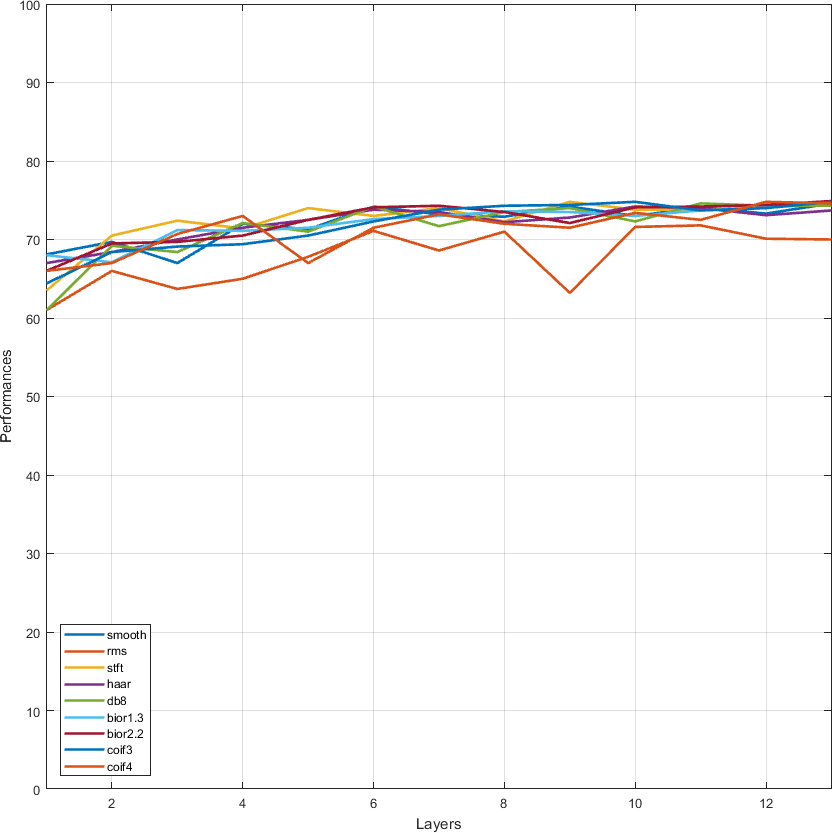
\includegraphics[width=14cm,center,keepaspectratio]{figures/sym4sym8}
   \caption{Average performances of networks from 1 to 13 layers, five neurons each. Each network was trained with the concatenation of sym4sym8 data and tested with 9 other features. The colors represent the names of the features and are shown in the legend box.}
   \label{fig:sym4sym8} 
\end{figure}
The following plot of the heatmap of the Table \ref{table:sym4sym8_1-5layers} is helping to give us a better visualization on which features had the best improvement over the increase of the layers of the neural networks.
\begin{figure}[h!]
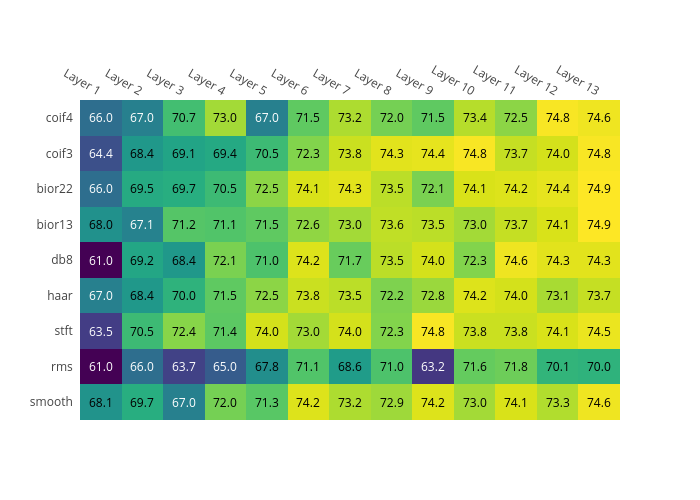
\includegraphics[width=17cm,center,keepaspectratio]{figures/accuracy_heatmap}
   \caption{Heatmap with the detection accuracies}
   \label{fig:accuracy_heatmap} 
\end{figure}
\section{Final evaluation}
To conduct the final evaluation we take the best parameters derived from the previous experiments for the adjustment of the parameters.\\
As we can see \ref{fig:sym4sym8} the rms feature does not perform so well as the other features. We will avoid to use 13 layers for our neural model as there is a risk of overfitting the train data. As we can notice the plateau with the best performances happen for 8 layers. Therefore, this is the number we will use for the final neural model. The features we will choose for the feature extraction are going to be db8, bior2.2, coif3, as they are the features with the best performances for 8 layers. We will evaluate the new finger gestures with a neural model which will consist of 8 layers and will train it with the triplet of sym4 and sym8 and one of the following best performed features for 8 layers: db8, bior2.2 and coif3.\\
We acquired new signals from the forearms of 21 subjects with age between 20-30. The new finger gestures we classify are the following:
The detection accuracies of the new gestures are listed below:
\begin{table}[h!]
\renewcommand{\arraystretch}{1.2}
\centering
\begin{tabular}{ |p{1.7cm}||p{1.1cm}|p{1.1cm}|p{1.1cm}|}
 \hline
 \multicolumn{4}{|c|}{sym4sym8} \\
 \hline
 Gestures  & db8 & bior2.2 & coif3 \\
 \hline
 G1 & $64.5\%$ & $74.6\%$ & $50.1\%$ \\
 G2 & $73.7\%$ & $69.6\%$ & $62.7\%$ \\
 G3 & $68.8\%$ & $68.3\%$ & $66.1\%$ \\
 G4 & $58.2\%$ & $64.4\%$ & $62.6\%$ \\
 G5 & $58.1\%$ & $51.3\%$ & $52.0\%$ \\
 G6 & $74.5\%$ & $75.2\%$ & $72.0\%$ \\
 G7 & $54.4\%$ & $53.1\%$ & $56.0\%$ \\
 G8 & $63.8\%$ & $74.2\%$ & $62.7\%$ \\
 G9 & $62.8\%$ & $57.3\%$ & $70.0\%$ \\
 G10 & $61.8\%$ & $74.7\%$ & $65.0\%$ \\
 G11 & $73.1\%$ & $68.2\%$ & $70.0\%$ \\
 G12 & $55.7\%$ & $71.2\%$ & $52.2\%$ \\
 G13 & $63.5\%$ & $73.2\%$ & $67.6\%$ \\
 G14 & $54.8\%$ & $50.8\%$ & $73.0\%$ \\
 \hline
\end{tabular}
\caption{Detection accuracies for extension and flexion of finger gestures with calibrated EMGs and trained with a neural network with 8 hidden layers and 5 hidden neurons in each layer.}
\label{table:sym4sym8_8layers}
\end{table}
The total number of neural nets that had to be trained were 42. The duration of the training all of them lasted for 5.2 days. The average time to train every neural net was 2.9 hours. 